\section{Presentation Logic Layer}
The site will be divided into two main areas, administration area and customer area, as follows:
\begin{itemize}
    \item \textbf{Administration area}: allows the staff member (front office users and manager) to have an overview of the hotel information.
    	\begin{itemize}
    			 \item \textbf{Front office users}: 
    			 \begin{itemize}
    			 	\item can add a new booking;
					\item can see only currently booking and sooner booking, grouped by rooms;
    			 \end{itemize}
    			 \item \textbf{Manager}: 
				\begin{itemize}
					\item can add a new booking;
					\item can see past booking (download a log), currently booking and sooner booking, grouped by rooms;
					\item can view payment status of the booking (pending list and confirmed list) and the payments methods of customers;
					\item can manage the front office users (create one, edit information, delete one, send reset password link);
					\item can view the information about front office users (like the last access);
				\end{itemize}    			 
    	\end{itemize}
    \item \textbf{Customers area}
    \begin{itemize}
	    \item \textbf{Homepage}: contains general information about the hotel, pictures and short descriptions about the different types of rooms and activities. Including a link to the login/registration page;
	    \item \textbf{Log in page}: allows customers, manager and front office users, to login into the web application;
	    \item \textbf{Registration page}: allows registration of customers user;
	    \item \textbf{Personal profile}: allows the customer to check its personal information, manage its booking - with two different buttons, one for starting a new booking procedure, and the other one for deleting a previous booking -, and choose the payment methods; 
	    \item \textbf{Booking page}: allows the customer to book a room for one or more guests, select the type of room and add some requests;
    \end{itemize}
  
\end{itemize}
\pagebreak
%For the main pages put a draft and describe it in detail.
\subsection{Administration Area}
Front office users and manager have a common administration interface, with the difference that some links and some buttons can only be used by the manager and not by the front office users, who will not be allowed to access via a message "access denied" error.
\input{sections/PLL/ManagerPage}
\subsection{Front office}
The administration interface of a front office user is basically the same as that of the manager, with the difference that some settings are not accessible.
The most different page is the homepage. The front office user sees the same manager homepage, but he cannot see the list of other users with their last accesses and therefore his homepage is only divided into two macro areas. In the first one he can see an overview of the latest news, such as the number of new bookings with some details about that. In the second one a list with the currently bookings and their relative details is shown.
Based on the pages that make up the manager interface, a front office user does not have the permissions to access to the payments page, users management page and every download log button present in all pages.
\begin{figure}[H]
	\centering
	%\label{fig:manager-index}
	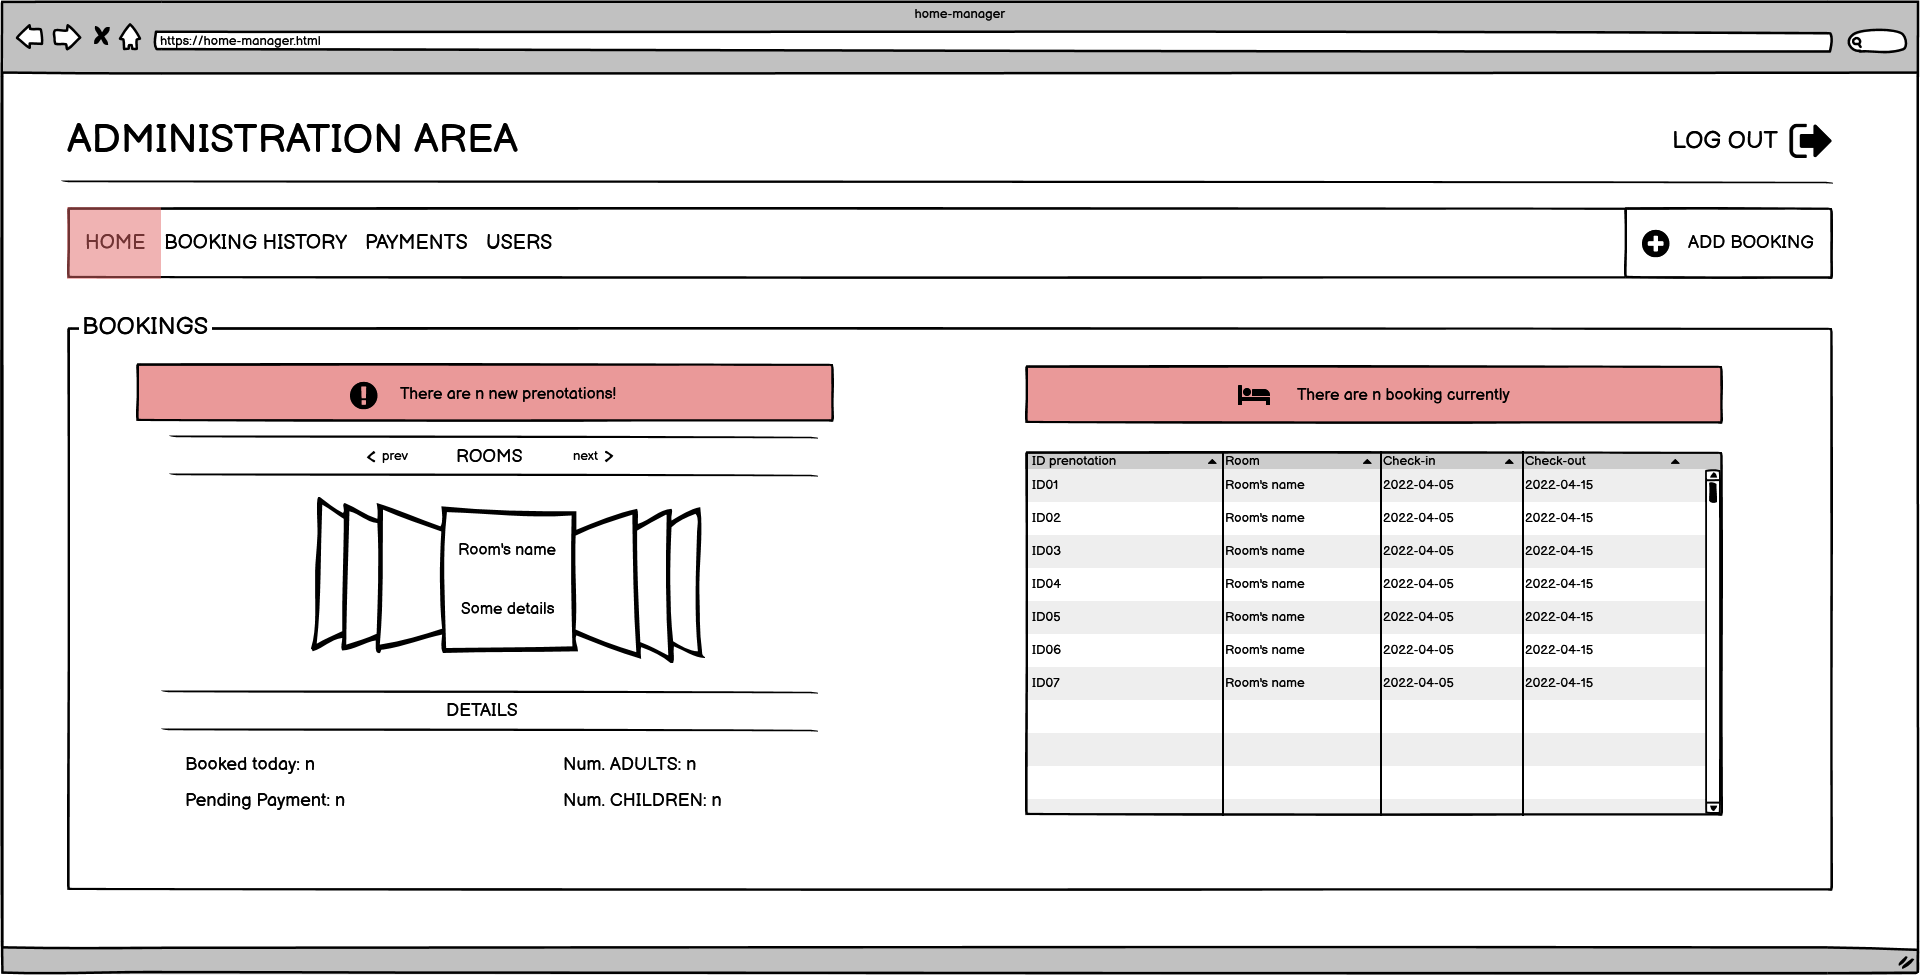
\includegraphics[height=7.5cm]{images/frontOffice-index.png} 
	\caption{Front office user homepage}
\end{figure}

\subsection{Customers Area}
The pages that make up the customer area are now described. 
\par \noindent A guest user can do with the booking procedure, but to complete it, a registration is required. 
\subsection{Homepage}
Different sections are created within the homepage to keep all the information easily available. One section is used for displaying information about the hotel itself. Another section summarises the types of rooms a potential customer can choose from, with different images and the last section contains the contact information of the hotel with a given email address and phone number. From this page it is possible to access to the page to login or register, if there is a new costumer.
\begin{figure}[H]
	\centering
	%\label{fig:manager-index}
	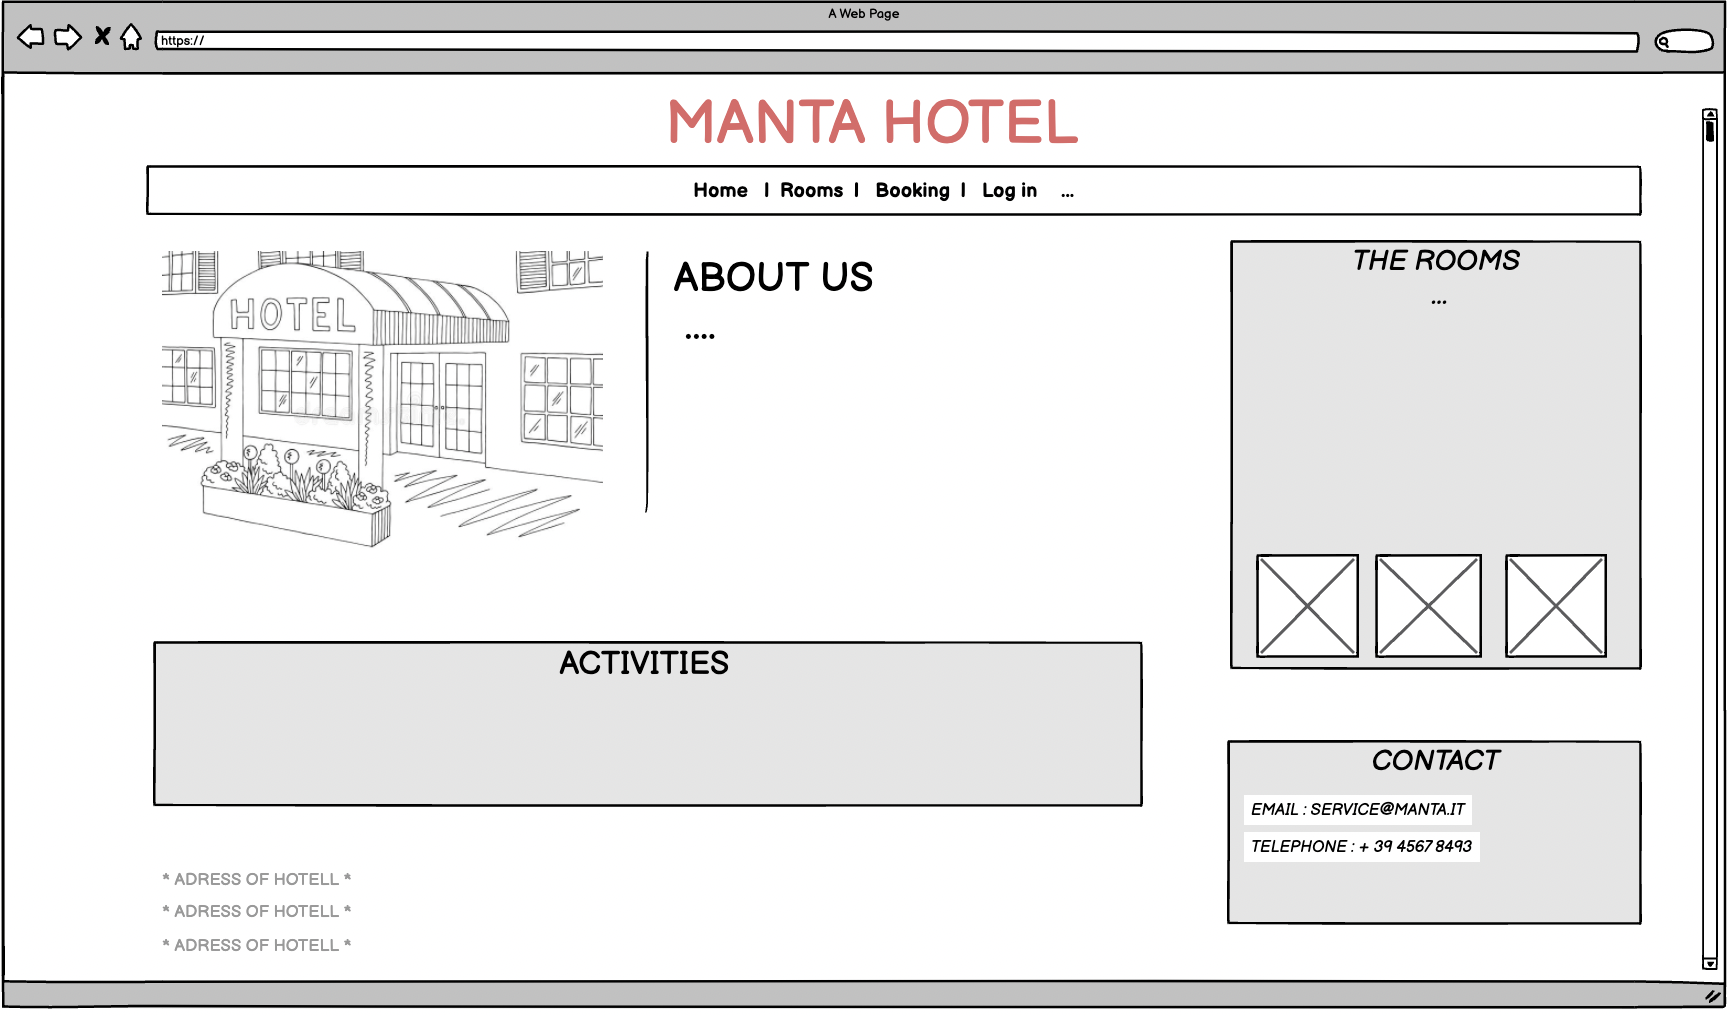
\includegraphics[height=7.5cm]{images/homepage_main.png} 
	\caption{Customers area: Homepage}
\end{figure}
\subsection{Booking page}
The booking procedure is held through six steps divided into two pages. 
\par \noindent In the first page there are three subsections: the first one is used to decide the date of arrival and departure with a possibility to add some requests in the specific window, the second one is used to select the number of rooms and guests, the third subsection is reserved to the selection of the room, presented as a carousel with the type and the description of each room, it is possible to use the "prev" and "next" button to navigate the carousel.
\par \noindent The second page displays three steps to complete the booking. The first section is dedicated to the insert guest information, some of the fields i.e. phone number and email are requested only for people over age of 18. It is possible to add different guests by using the plus button. The next section shows the summary of the booking with all the details and the last one directs to the payment. 

\begin{figure}[H]
	\centering
	%\label{fig:manager-index}
	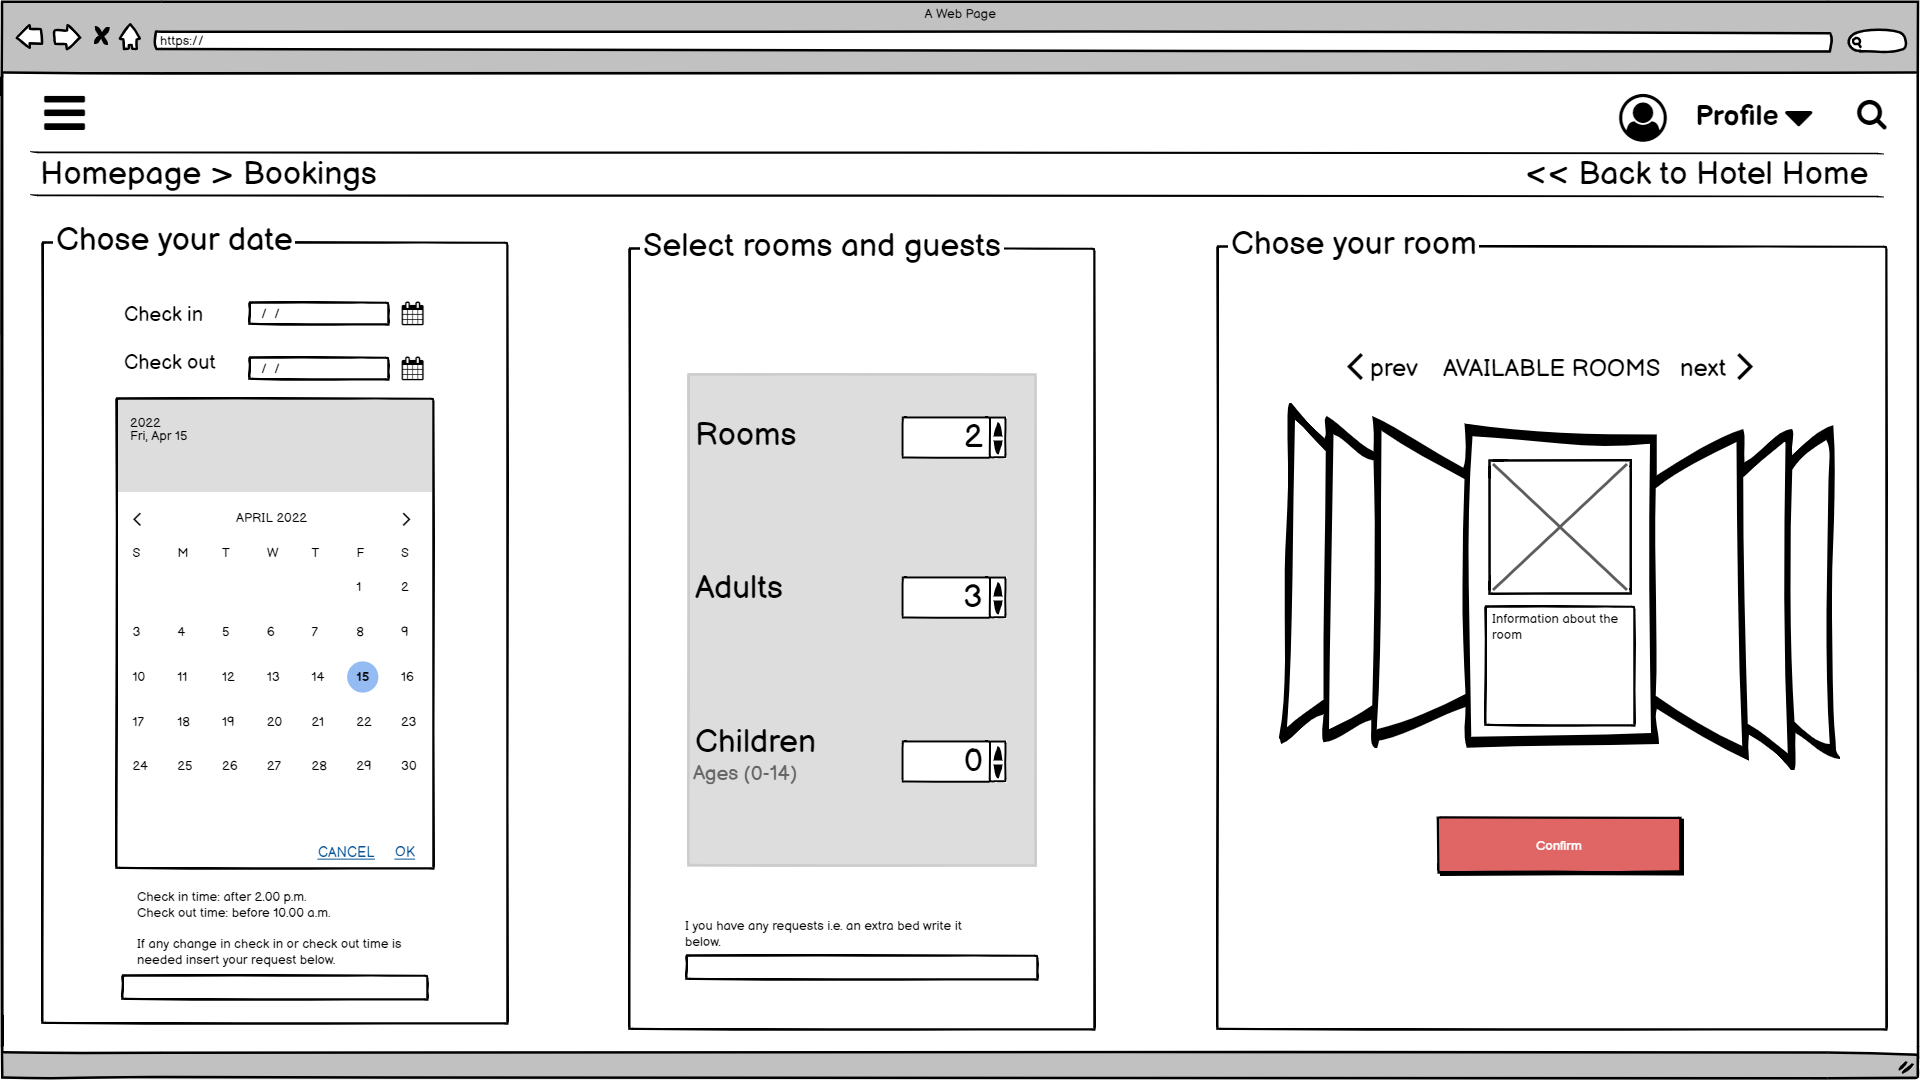
\includegraphics[height=7.5cm]{images/Booking.png} 
	\caption{Booking pages: first page}
\end{figure}
\begin{figure}[H]
	\centering
	%\label{fig:manager-index}
	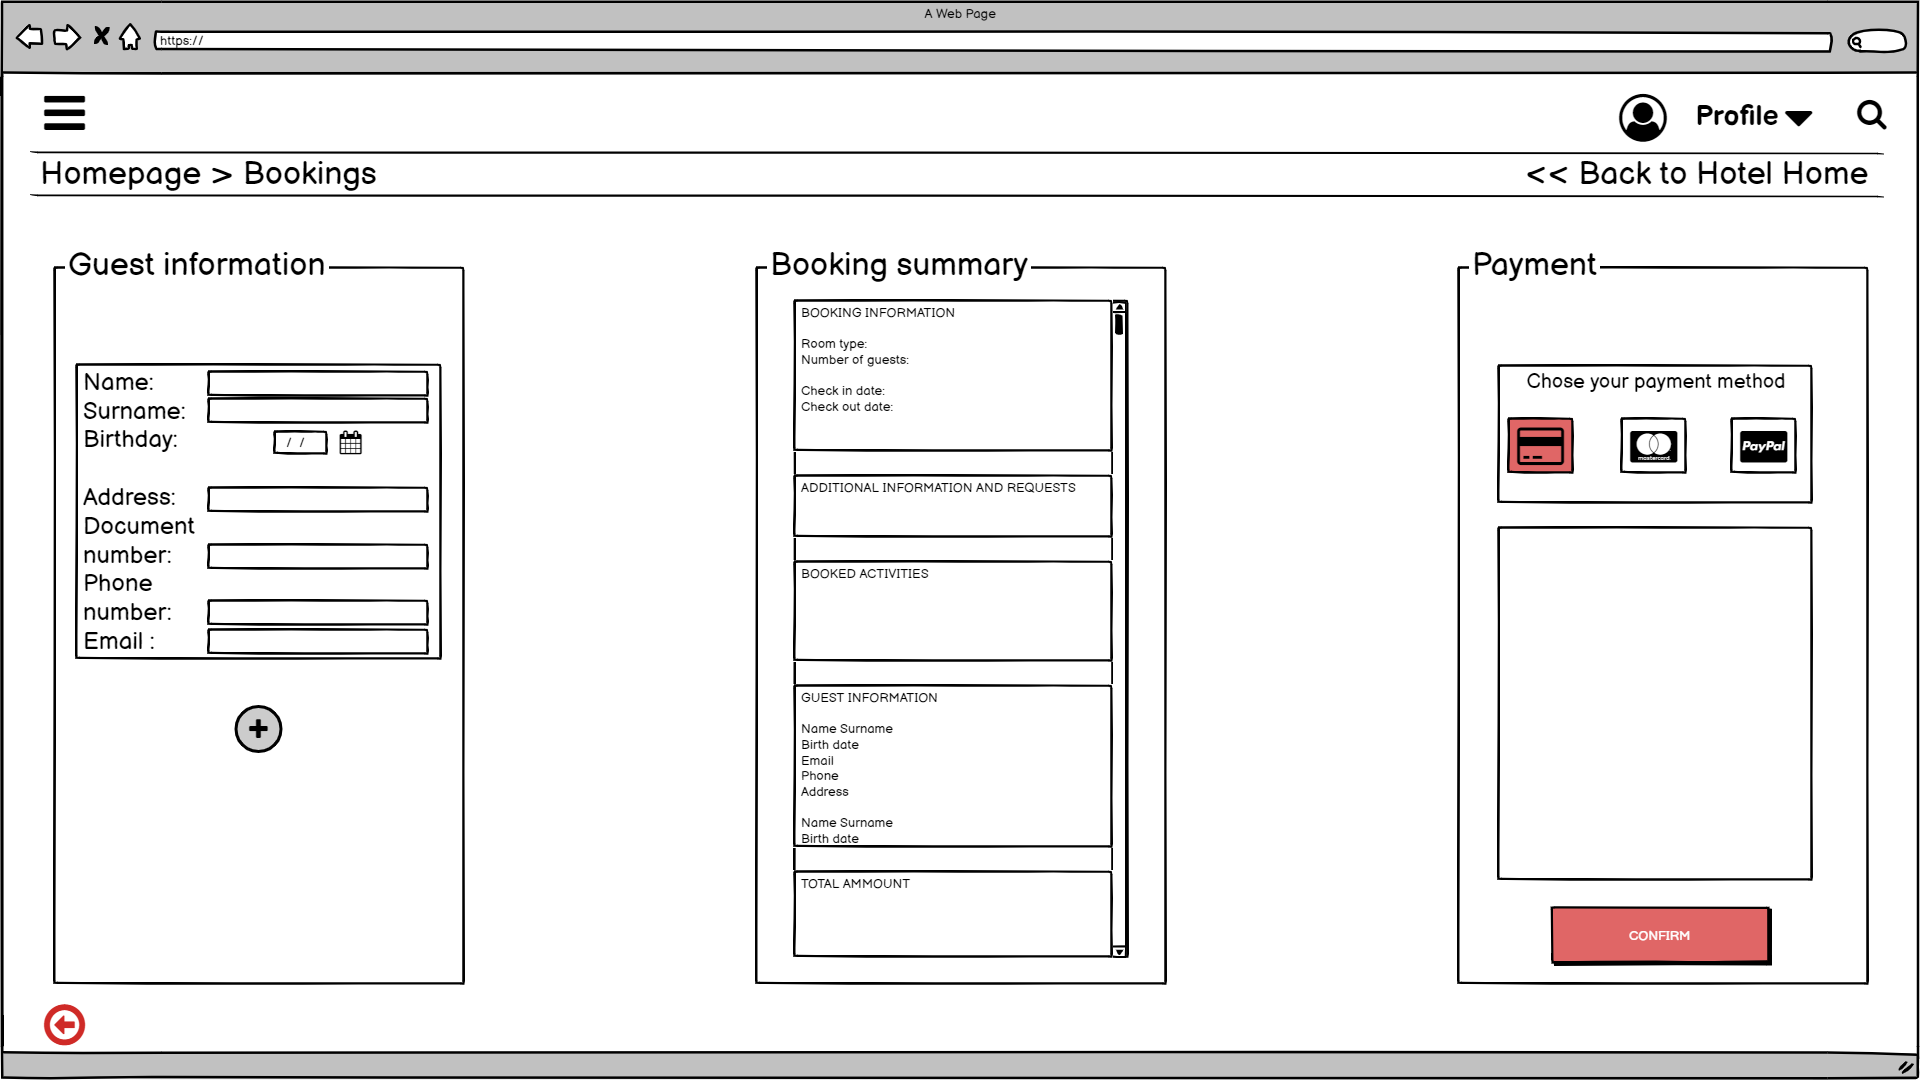
\includegraphics[height=7.5cm]{images/booking_2.png} 
	\caption{Booking pages: second page}
\end{figure}
\pagebreak
\subsection{Log in and registration page}
\par The log in page allows both customers and users (staff members in the reception) to log in and use the Manta Hotel web application, with only their username and password. 
\par If one is not a user, one can register by clicking the registration link. This will send the soon to be user to a registration form where one has to fill out all the necessary information in order to register. 
\begin{figure}[H]
	\centering
	%\label{fig:manager-index}
	\includegraphics[height=7.5cm]{images/HomePage_Login.png} 
	\caption{Customers area: Login page}
\end{figure}
\begin{figure}[H]
	\centering
	%\label{fig:manager-index}
	\includegraphics[height=7.5cm]{images/HomePage_Register.png} 
	\caption{Customers area: Registration page}
\end{figure}

\subsection{Personal page}
In the personal area page the customer can navigate through personal information, past and current bookings (check symbol button), it is possible to book a new room (+ button) and chose different payment methods. The bookings can be sorted by date. There are two buttons to check the past bookings and start a new one. It is also possible to open a tend from the profile button in the right top corner in order to check the settings, help section or log out.

\begin{figure}[H]
	\centering
	%\label{fig:manager-index}
	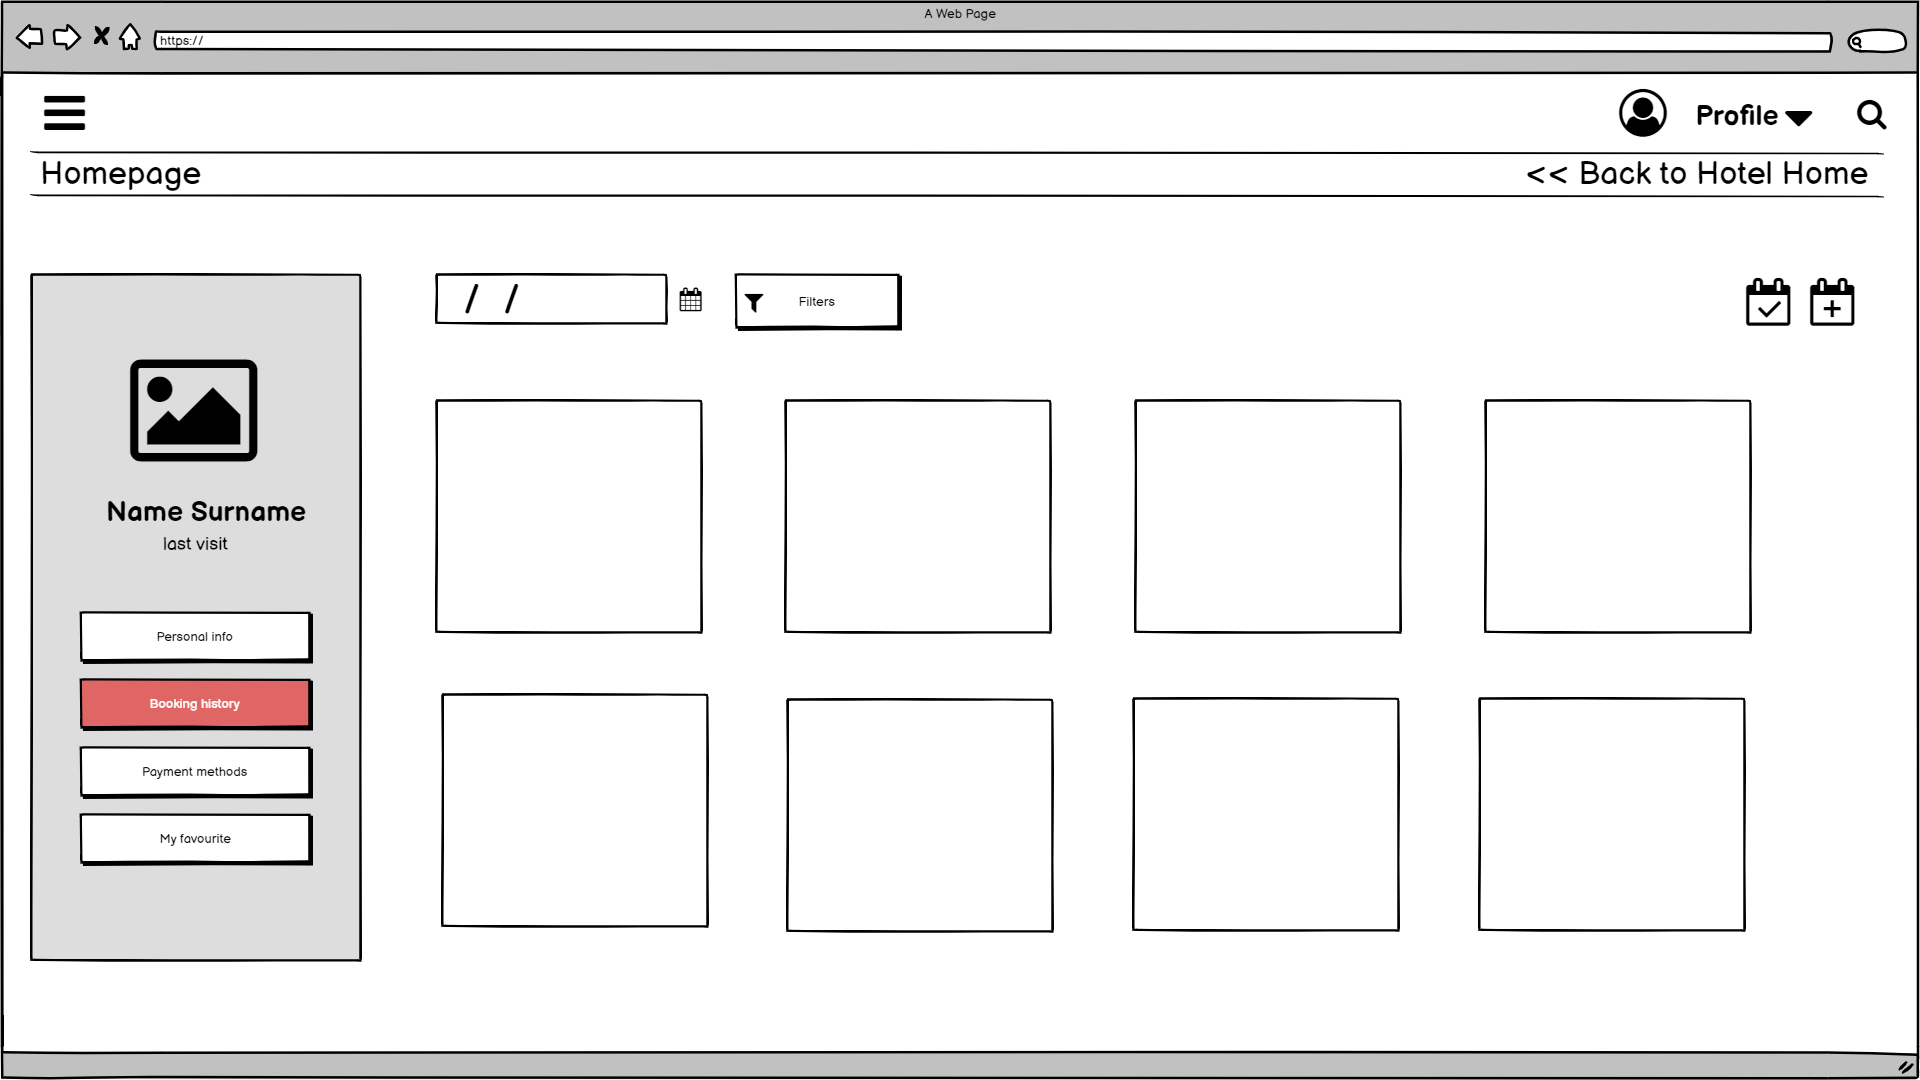
\includegraphics[height=7.5cm]{images/personal_1.png} 
	\caption{Customers page}
\end{figure}
\begin{figure}[H]
	\centering
	%\label{fig:manager-index}
	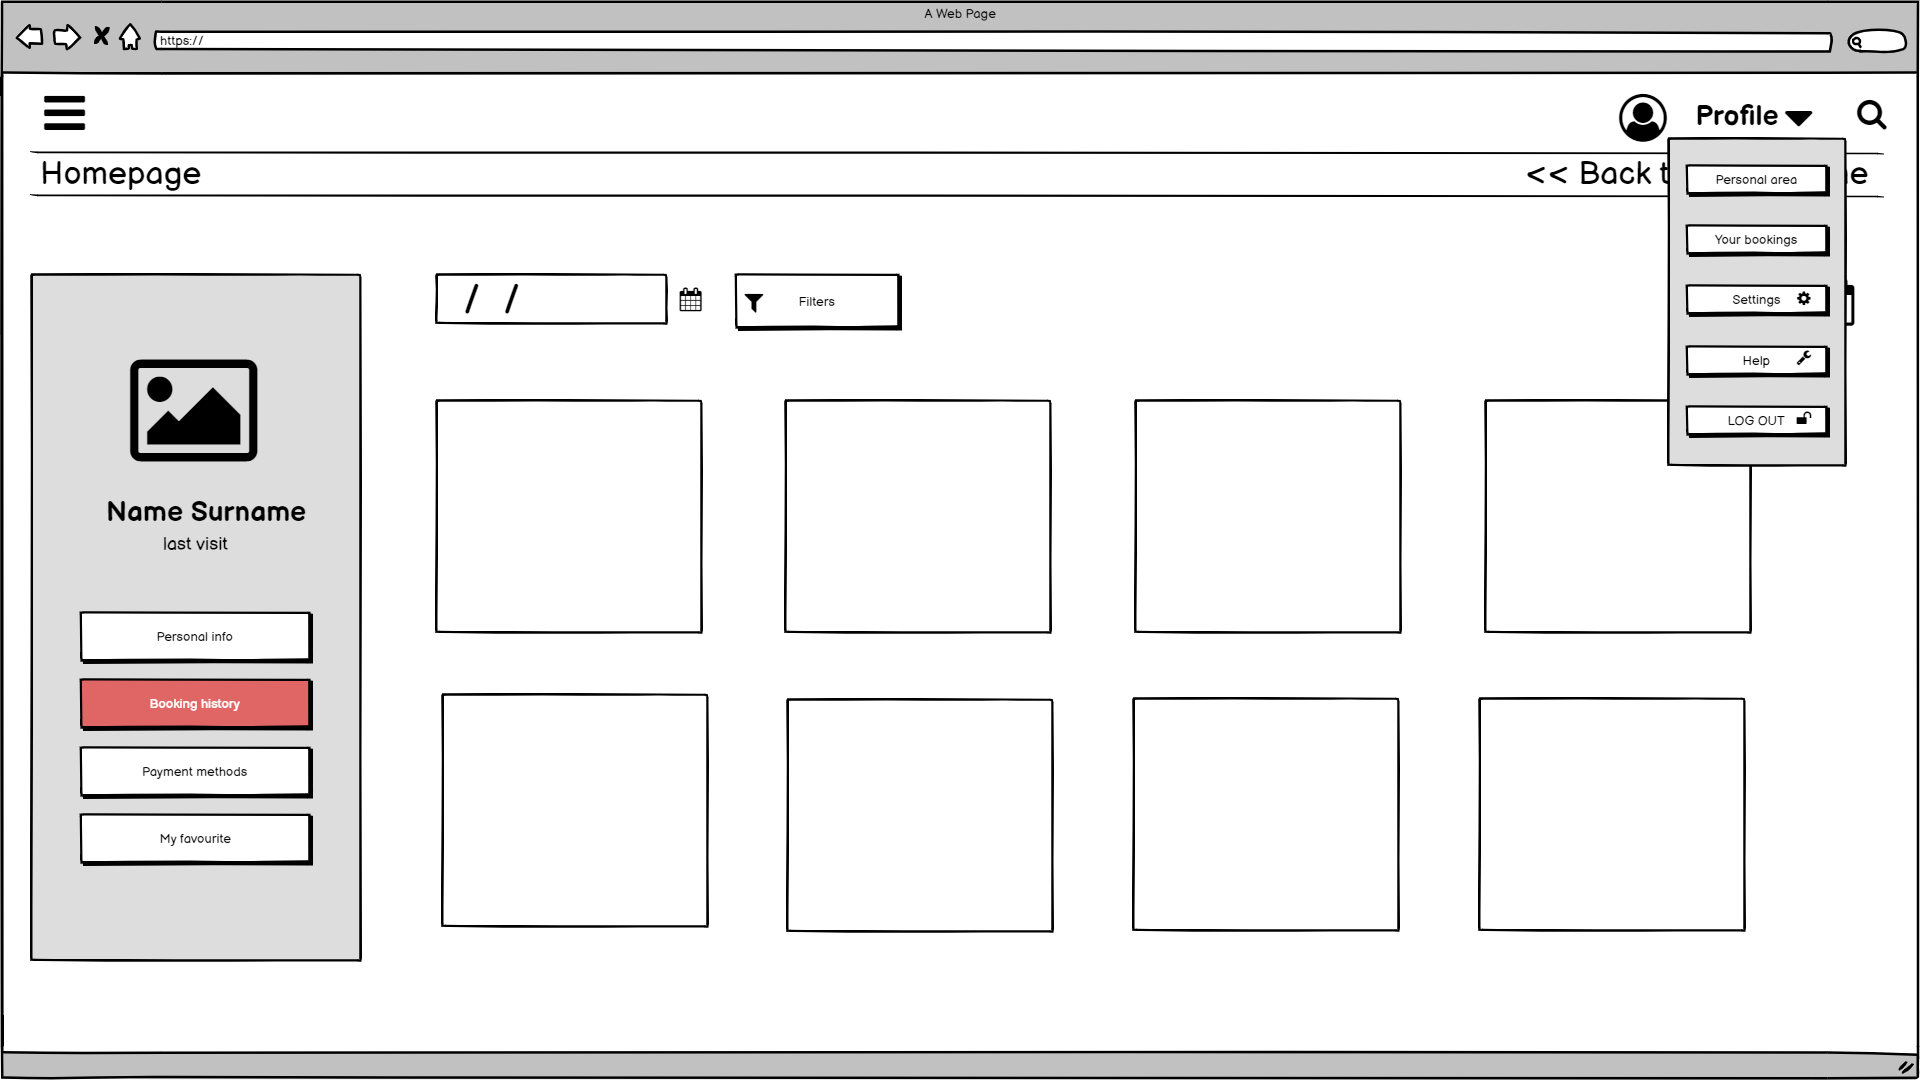
\includegraphics[height=7.5cm]{images/personal_2.png} 
	\caption{Customers page: tend menu}
\end{figure}

